\documentclass{article}
\usepackage[utf8]{inputenc}
\usepackage[margin=2.3cm]{geometry}
\usepackage{amsmath, amssymb}
\usepackage{float}
\usepackage{hyperref}
\usepackage{natbib}
\usepackage{booktabs}
\usepackage{graphicx}
\usepackage{algorithm}
\usepackage{algpseudocode}
\usepackage{titlesec}
\titlespacing*{\section}{0pt}{2.2ex plus 1ex minus .2ex}{1.4ex plus .2ex}
\titlespacing*{\subsection}{0pt}{2.0ex plus 1ex minus .2ex}{1.0ex plus .2ex}

\newcommand{\eff}{k_{\mathrm{eff}}}
\newcommand{\mse}{\mathrm{MSE}}
\newcommand{\nmse}{\mathrm{NMSE}}

\title{Equation Discovery for Extrapolation:\\
Systematic Skeleton Search with a Projected Polynomial Background}
\author{Mika Ben Brückner}
\date{\today}

\begin{document}
\maketitle

\section{Introduction}
\label{sec:intro}

A central promise of machine learning is prediction \emph{beyond} the 
observed data, and standard regressors are remarkably bad at it: a polynomial
diverges at a rate dictated by its degree, a random forest predicts a
constant outside the convex hull of the training inputs, and a multi-layer
perceptron (MLP) extrapolates linearly. All three interpolate the data in
Figure~\ref{fig:demo} almost perfectly, yet all three fail immediately
outside the training domain. Symbolic regression (SR) offers a way out for
an important class of problems: many systems in science and engineering
can ultimately be described by comparatively simple closed-form equations, and if
the data-generating process \emph{is} such a formula $f$, recovering $f$ up to
symbolic equivalence yields exact extrapolation by construction. The price
is a hard combinatorial search over expression
space~\citep{DongZhongSurvey}, and when the data does \emph{not}
follow a formula expressible in the search language, SR has no
extrapolation advantage (Section~\ref{sec:discussion}).

\begin{figure}[H]
  \centering
  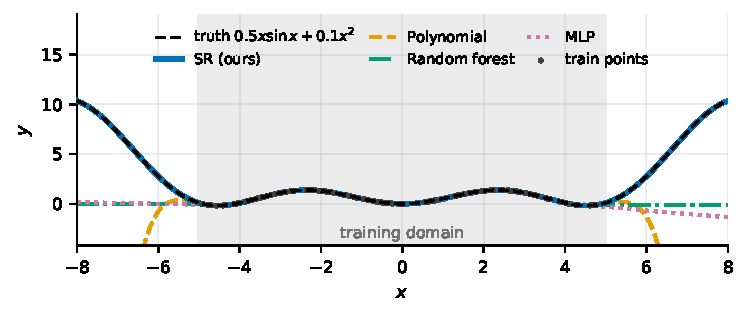
\includegraphics[width=.66\linewidth]{../results/figs/demo.pdf}
  \caption{Extrapolation on $f(x)=0.5x\sin x+0.1x^2$ (128 noise-free training
  points on $[-5,5]$). The baselines fit the training domain but fail outside
  it. Our method recovers the formula exactly
  ($\hat f(x) = 0.5\,x\sin x + 0.1\,x^2$) and extrapolates perfectly.
  Its curve coincides with the dashed ground truth.}
  \label{fig:demo}
\end{figure}

\paragraph{Problem statement.}
Let $f:\mathbb{R}^d\to\mathbb{R}$ be an unknown formula over a known operator
alphabet. We observe $N_{\mathrm{train}}$ samples
$(x_i, y_i)$ with $x_i \sim \mathrm{Unif}([-a,a]^d)$ and
$y_i = f(x_i) + \varepsilon_i$, $\varepsilon_i \sim
\mathcal{N}(0,\sigma^2)$. The goal is a model $\hat f$ that minimizes the
error on test points sampled \emph{strictly outside} the training domain,
$x \sim \mathrm{Unif}([-b,b]^d \setminus [-a,a]^d)$ with $b > a$:
\begin{equation}
  \mse_{\mathrm{test}} \;=\; \frac{1}{N_{\mathrm{test}}}
  \sum_{i=1}^{N_{\mathrm{test}}} \bigl(\hat f(x_i) - f(x_i)\bigr)^2 .
  \label{eq:msetest}
\end{equation}

This report describes (i) an SR algorithm combining an unbiased,
complexity-ordered search over expression skeletons in the spirit
of~\citet{Kahlmeyer} with two extrapolation-specific components: a polynomial
background solved in closed form by variable projection (generalizing linear
scaling~\citep{Keijzer}), and model selection by \emph{extrapolation-shaped}
cross-validation, (ii) a synthetic generator that samples random formulas by
a dice roll over operators, and (iii) experiments mapping out where the
method beats polynomial, random-forest, and MLP baselines, and where it
breaks.

\section{Approach}
\label{sec:approach}

\paragraph{Related work.}
SR systems search by genetic programming~\citep{PySR}, by gradient descent
through operator layers~\citep{NeuralSR,SymbolNet}, or by continuous
relaxation~\citep{ParFam}, all biasing the search~\citep{DongZhongSurvey} in
ways that are hard to check~\citep{Kahlmeyer}. We adopt the assumption-free stance
of~\citet{Kahlmeyer}, whose search is unbiased but randomized, and make it
\emph{systematic}: enumerate small expressions in order of size.

\subsection{Model assumptions}
\label{sec:model}

\paragraph{Expression skeletons.}
We search over \emph{skeletons}: expression trees whose internal nodes carry
operators from
$\mathcal{U} = \{\sin,\cos,\exp,\log,\sqrt{\cdot},(\cdot)^2\}$ (unary) and
$\mathcal{B} = \{+,-,\times,\div\}$ (binary), and whose leaves are either
input variables $x_j$ or constant placeholders $c$. A skeleton $u$ with $p$
placeholders defines a parametric family $u_\theta$, $\theta \in
\mathbb{R}^p$. Following~\citet{Kahlmeyer}, the only structural assumption we
place on the search space is that it contains \emph{small} expressions: the
\emph{core complexity} $k(u)$ is the number of operator nodes, and the search
proceeds in order of increasing $k$. We use \emph{protected} operators
$\log|t|$ and $\sqrt{|t|}$ so that they impose no domain restrictions.
Division is left unprotected, so skeletons using it may have poles, and
invalid evaluations are penalized during fitting.

\paragraph{Regression model.}
A skeleton is turned into a regressor by attaching a linear \emph{polynomial
background},
\begin{equation}
  \hat f(x) \;=\; \alpha\, u_\theta(x) \;+\; \textstyle\sum_{j=1}^{m} \beta_j\, m_j(x),
  \label{eq:model}
\end{equation}
where $\{m_j\} = \{1\} \cup \{x_j^q : q \le \mathrm{deg}\}$ (plus $x_0x_1$ for
$d=2$) are fixed monomials, $\mathrm{deg} \in \{2,3\}$ by Section~\ref{sec:config}. The background, a generalization of linear
scaling~\citep{Keijzer} from $\{1\}$ to a monomial basis, is the crucial
ingredient: the core $x\sin x$ explains Figure~\ref{fig:demo} up to a
polynomial trend, so with~\eqref{eq:model} it is the best of the $69$
skeletons at $k=2$, at machine precision. Under plain linear scaling it
still ranks first but leaves $40\%$ of the variance unexplained, and without
the background it drops to rank $24$ and is pruned.
The \emph{total complexity} of a fitted model
is $C = k(u) + \#\{j \ge 2: \beta_j \neq 0\}$, core operators plus active
non-intercept background terms.

\subsection{Parameter learning}
\label{sec:learning}

For a fixed skeleton $u$ the parameters split into a nonlinear part $\theta$
and a linear part $(\alpha,\beta)$. We exploit this by \emph{variable
projection}: for given $\theta$, the optimal linear coefficients are the
ordinary least-squares solution
\begin{equation}
  (\alpha^*,\beta^*)(\theta) \;=\; \arg\min_{\alpha,\beta}
  \bigl\lVert y - \alpha\, u_\theta(X) - M\beta \bigr\rVert_2^2,
  \qquad M_{ij}=m_j(x_i),
  \label{eq:varpro}
\end{equation}
computed in closed form. Substituting back leaves a nonlinear least-squares
problem in $\theta$ only, $\min_\theta \lVert r(\theta)\rVert_2^2$ with
$r(\theta) = y - \alpha^*(\theta)\,u_\theta(X) - M\beta^*(\theta)$, solved by
a trust-region solver (finite-difference Jacobians) from multiple starts:
$\theta^{(0)} = \mathbf{1}$ and one draw from $\mathcal{N}(0, 2^2 I)$
(two draws for $p\ge3$). Non-finite predictions are mapped to a large constant to
penalize invalid parameter regions. Skeletons with $p > 6$ placeholders are
discarded. Selected models are finally \emph{sparsified}: background terms
with contribution $|\beta_j|\,\mathrm{std}(m_j) <
10^{-4}\,\mathrm{std}(y)$ are removed and the linear part refitted.

\subsection{Search: exhaustive enumeration, then a diversity-aware beam}
\label{sec:search}

Semantically equivalent skeletons waste search budget, so trees are mapped
to a canonical representative. Constant subtrees fold into a placeholder
($\sin(c) \to c$). Associative chains are flattened, sorted, and allowed at
most one constant term. Parameter-absorbing compositions are rejected
($t-c$, $t/c$, $e^{t+c}$, $\log|ct|$, $\sqrt{|ct|}$, $(ct)^2$, $\log e^t$,
$t+t$, $t\cdot t$, $t-t$, $t/t$).
Operator aliases of the absolute value ($e^{\log|t|} = (\sqrt{|t|})^2 =
|t|$) are kept only as $\sqrt{t^2}$. For $d=1$ this leaves
$1, 6, 69, 890, 12\,769$ skeletons with $k = 0,\dots,4$ operator nodes.

These rules only remove duplicates they can \emph{prove}. Many more
skeletons are numerically redundant with respect to \eqref{eq:model}: since
$\alpha$ and the intercept are free, cores agreeing up to an affine
transform of their output are interchangeable, and with the full background
so are cores differing by a background polynomial. We detect this with an
\emph{evaluation fingerprint}: each skeleton is evaluated on $24$ fixed
probe points for $3$ generic parameter draws, the monomial basis is
projected out (\emph{background}) or not (\emph{affine}), and the normalized
result is hashed. A skeleton whose
fingerprint was seen is skipped without fitting. The filter is heuristic in
both directions: it can merge families that agree only on the probe points,
and prune cores that are redundant alone but serve as intermediates. It is
therefore validated in Section~\ref{sec:config}.

Search runs in two phases (Algorithm~\ref{alg:search}). Phase~1 fits
\emph{every} canonical skeleton up to $k_{\mathrm{ex}}$ ($3$ or $4$ for $d=1$,
$2$ or $4$ for $d=2$). This is an unbiased search in the sense of~\citet{Kahlmeyer},
placing the method in the \emph{deterministic} branch of the taxonomy
of~\citet{DongZhongSurvey}, whose known trade-off (global optimality at
exponentially growing cost) is exactly the behaviour we quantify in
Section~\ref{sec:main}. Phase~2
grows skeletons one operator at a time with a beam. Expansions of a parent
are all canonical trees obtained by replacing a leaf with a depth-one
subtree or combining any node with a fresh leaf or unary wrapper. Ranking
parents purely by training loss makes the beam greedy, so parents are chosen
\emph{round-robin across root-operator groups} in order of loss, plus $5$
uniformly random survivors ($\varepsilon$-greedy). To bound cost, constants
are fitted on a random subsample of $64$ points during the search and
refitted on all of them afterwards. The output is a \emph{Pareto front}
$\mathcal{F} = \{\hat f_k\}$: the best model per core complexity
$k \le k_{\max}$, kept only where the training loss strictly improves.

\begin{algorithm}[t]
\caption{Complexity-ordered skeleton search and parameter learning. Both loops
stop as soon as $\min \mathcal{F} < 10^{-10}\,\mathrm{Var}(y)$.}
\label{alg:search}
\begin{algorithmic}[1]
\Require data $(X,y)$, $64$-point subsample $(X_s,y_s)$, operators
$(\mathcal{U},\mathcal{B})$, limits $k_{\mathrm{ex}}, k_{\max}$, beam width $B$
\State $\mathcal{F} \gets \emptyset$ \Comment{front: best model per core complexity}
\For{$k = 0,\dots,k_{\mathrm{ex}}$} \Comment{Phase 1: exhaustive}
  \State $L_k \gets$ all canonical skeletons with $k$ operator nodes
  \State \Call{Fit}{$u,X_s,y_s$} for each $u \in L_k$; update $\mathcal{F}$
\EndFor
\For{$k = k_{\mathrm{ex}}+1,\dots,k_{\max}$} \Comment{Phase 2: beam}
  \State $P \gets$ round-robin top-$B$ of $L_{k-1}$ by loss across root
  operators $\cup$ 5 random
  \State $L_k \gets$ canonical one-operator expansions of $P$ (deduplicated)
  \State \Call{Fit}{$u,X_s,y_s$} for each $u \in L_k$; update $\mathcal{F}$
\EndFor
\State refit $\mathcal{F}$ on all training points; sparsify; return Pareto-optimal $\mathcal{F}$
\Procedure{Fit}{$u,X,y$} \Comment{variable projection, Section~\ref{sec:learning}}
  \State $\theta^\star \gets \arg\min_\theta \lVert r(\theta)\rVert_2^2$ by multi-start trust-region NLS,
  where $r(\theta) = y - P(\theta)P(\theta)^{+}y$ and $P(\theta) = [\,u_\theta(X)\mid M\,]$
  \State \Return $\theta^\star$, \; $(\alpha,\beta) = P(\theta^\star)^{+}y$, \; loss $\lVert r(\theta^\star)\rVert_2^2/N$
\EndProcedure
\end{algorithmic}
\end{algorithm}

\subsection{Model selection: extrapolation-shaped cross-validation}
\label{sec:selection}

The front $\mathcal{F}$ ranges from underfit to overfit models. Picking by
training loss would always return the most complex one. Because our target
is~\eqref{eq:msetest} rather than interpolation error, we validate the way we
will be tested: training points are ranked by their sup-norm distance from
the domain center, and for each quantile $q \in \{0.5, 0.6, 0.7, 0.8\}$ a
fold is formed that refits each candidate's constants on the inner $q$
fraction and validates on the outer ring, giving cross-validation over
\emph{extrapolation horizons}. With $\mathrm{cv}_{k,f}$ the validation MSE of
$\hat f_k$ on fold $f \in F$, candidates are scored by
$s_k = \tfrac{1}{|F|}\sum_f \log \mathrm{cv}_{k,f}$, and the winner is chosen
by the one-standard-error rule~\citep[\S7.10.1]{ESL}: among all candidates with
$s_k \le s_{k^\dagger} + \widehat{\mathrm{se}}(s_{k^\dagger})$, where
$k^\dagger$ is the score minimizer and $\widehat{\mathrm{se}}$ its standard
error across folds, the one with the smallest total complexity $C_k$ is
selected and refitted on all training data. This makes the choice robust on
training-loss plateaus, where CV differences between models are mostly noise.
Candidates that diverge just outside the training box are removed
beforehand by the growth guard motivated in Section~\ref{sec:analysis}.
All hyperparameters of the baselines~\citep[Ch.~3, 11, 15]{ESL} are tuned on the \emph{same}
folds (Section~\ref{sec:setup}). Ridge and the MLP run on standardized
features, ours needs no scaling, so the comparison is fair.

\subsection{Limits of the model}
\label{sec:limits}

The hypothesis space is bounded by $k_{\max}$ ($7$ core operators for $d=1$)
and by the beam: formulas whose subterms only pay off jointly (e.g.\ the
damped oscillation $e^{-c|x|}\cos(cx)$, $k=7$) can be missed though representable. Protected $\log$ and $\sqrt{\cdot}$ extend past
their natural domains~\citep{Keijzer}. Unprotected division admits poles that make fitting
and evaluation ill-conditioned. Constant fitting is non-convex. Multi-starts
mitigate but do not eliminate local minima ($\sin$ frequencies are the
classic failure). Finally, the background biases the method towards ``scaled
core $+$ polynomial'' structure. Formulas like $\sin(x_0x_1)\log|x_0|$
receive no help from it.

\section{Experiments}
\label{sec:experiments}

\subsection{Setup}
\label{sec:setup}

\paragraph{Data generator.}
Ground truths are sampled by a dice roll: a random tree with a
prescribed number of operator nodes over one of three alphabets
($\mathcal{O}_{\mathrm{poly}}$: $\{+,-,\times,(\cdot)^2\}$;
$\mathcal{O}_{\mathrm{trig}}$: $\mathcal{O}_{\mathrm{poly}}
\cup \{\sin,\cos\}$; $\mathcal{O}_{\mathrm{full}}$: all ten operators), with
leaves $x_j$ (probability $0.7$) or constants from
$\pm\,\mathrm{Unif}([0.2, 3])$. A formula is rejected if, on a dense grid over
$[-8,8]^d$, it produces invalid values, $\max|f| > 10^4$ or
$\mathrm{std}(f) < 10^{-3}$, if it ignores a variable, or if it has $\ge 3$
dice operators but is numerically affine. Because dice-rolled trees often
simplify (e.g.\ $x\,(x - x - x)^2 = x^3$), analyses bin by the
\emph{effective complexity} $\eff$, the operator count of the
\texttt{sympy}-simplified formula. Datasets use $N_{\mathrm{train}} = 128$,
$N_{\mathrm{test}} = 256$, $a = 5$, $b = 8$, and relative noise
$\sigma = \sigma_{\mathrm{rel}}\,\mathrm{std}(f(X))$.

\paragraph{Metrics.}
We report the normalized test error $\nmse = \mse_{\mathrm{test}} /
\mathrm{Var}(y_{\mathrm{test}})$, aggregated by medians (and IQRs) since
single blow-ups dominate means ($\nmse = 1 \approx$ predicting a constant),
and the \emph{recovery rate}~\citep{Kahlmeyer}: the fraction of runs whose
model matches the ground truth on a dense grid over $[-8,8]^d$ with relative
RMSE below $10^{-6}$, i.e.\ functional identity. Baselines are polynomial ridge
regression (degree $\le 8$, penalty on a grid), random forest (depth grid),
and an MLP (width/penalty grid), all tuned on the extrapolation-shaped folds
of Section~\ref{sec:selection}. Everything is seeded, and the two
commands in \texttt{README.md} reproduce all numbers.

\subsection{Search configuration}
\label{sec:config}

\begin{table}[t]
  \centering
  \caption{Search configurations on $48$ \emph{hard} datasets ($d{=}1$,
  $\mathcal{O}_{\mathrm{trig}}/\mathcal{O}_{\mathrm{full}}$, $4$--$8$ dice
  operators), varied one factor at a time around the default. Total time is
  a configuration's cost over all $48$ datasets. The
  last two rows arbitrate between all eleven configurations \emph{per
  dataset} by the cross-validated score $s_k$ of
  Section~\ref{sec:selection}, while ``oracle'' instead picks the smallest
  test error and is an upper bound. Both report the selected run only.}
  \label{tab:hyper}
  {\footnotesize\begin{tabular}{lcccc}
\toprule
Configuration & med.\ NMSE$_{\mathrm{test}}$ & Recovery & med.\ \#fits & med.\ time [s] \\
\midrule
default ($k_{\mathrm{ex}}{=}3$, no dedup, $B{=}15$, deg $2$) & $2.4\!\cdot\!10^{-30}$ & 67\% & 1783 & 5.2 \\
k\_ex=2 & $4.6\!\cdot\!10^{-30}$ & 62\% & 766 & 6.9 \\
k\_ex=4 & $5.0\!\cdot\!10^{-30}$ & 62\% & 2929 & 7.4 \\
dedup=affine & $3.1\!\cdot\!10^{-30}$ & 65\% & 1334 & 4.4 \\
dedup=background & $4.8\!\cdot\!10^{-30}$ & 69\% & 1280 & 6.3 \\
k\_ex=4+dedup & $8.6\!\cdot\!10^{-29}$ & 71\% & 1986 & 12.7 \\
beam=5 & $9.4\!\cdot\!10^{-22}$ & 62\% & 1535 & 5.7 \\
beam=40 & $2.4\!\cdot\!10^{-30}$ & 69\% & 2486 & 16.1 \\
poly\_deg=0 & $8.0\!\cdot\!10^{-29}$ & 62\% & 3282 & 53.8 \\
poly\_deg=1 & $3.1\!\cdot\!10^{-30}$ & 62\% & 2127 & 9.8 \\
poly\_deg=3 & $2.6\!\cdot\!10^{-30}$ & 71\% & 1364 & 6.8 \\
\midrule
CV-selected per dataset & $2.4\!\cdot\!10^{-30}$ & 79\% & 656 & 2.6 \\
oracle (best test error) & $1.2\!\cdot\!10^{-30}$ & 79\% & -- & -- \\
\bottomrule
\end{tabular}}
\end{table}

We first fix the search hyperparameters by cross-validation, on the same
extrapolation-shaped folds as Section~\ref{sec:selection} and never on test
data. Table~\ref{tab:hyper} reports a one-factor-at-a-time grid. Recovery
differences between the levels of a factor never exceed four of the $48$
datasets, so single rows indicate trends rather than resolved effects. Three observations drive
the final configuration. \emph{Deeper exhaustive
enumeration pays off, but only together with deduplication}: $k_{\mathrm{ex}}=4$
alone recovers $62.5\%$, below the default, but with deduplication it
reaches $70.8\%$ versus $66.7\%$ at $55\%$ of the
\emph{total} compute, although its \emph{median} run is slower. The extra level finds the formula in Phase~1 often enough to
skip the beam, and with it the multi-minute worst cases that dominate the
total. The \emph{background} is
confirmed as the decisive component: recovery is non-decreasing in its degree, and
cutting it back to plain linear scaling~\citep{Keijzer} ($\mathrm{deg}{=}0$)
makes the median search ten times slower, because it then rarely terminates
early. A \emph{wider beam} ($B=40$)
buys almost nothing at double the cost, confirming that the bottleneck is
the scoring of candidates rather than their number.

The CV-selected row of Table~\ref{tab:hyper} arbitrates over all eleven
configurations, not the deployed two. Since no single configuration
dominates, the final method runs a small \emph{portfolio} and keeps the
model with the better cross-validated score.
Two configurations, $(k_{\mathrm{ex}}{=}4$, dedup$)$ and
$(\mathrm{deg}{=}3)$, already reach $79.2\%$ (exactly the oracle rate of
the full grid, at a ninth of its cost) because an exactly recovered
formula drives its cross-validated error to numerical zero, a signal no
incorrect configuration can imitate. All following experiments use this
portfolio.

\subsection{Extrapolation error and recovery}
\label{sec:main}

\begin{table}[t]
  \centering
  \caption{Median $\nmse_{\mathrm{test}}$ (lower is better, $10^{-30}$ is exact
  recovery, $1$ is as bad as predicting a constant)
  and SR recovery rate, per operator alphabet and input dimension, from $25$
  ($d{=}1$) resp.\ $15$ ($d{=}2$) random formulas per alphabet--complexity
  cell, noise-free. Note that $d{=}2$ omits $\mathcal{O}_{\mathrm{poly}}$.}
  \label{tab:main}
  \begin{tabular}{lccccc}
\toprule
Setting & SR (ours) & Polynomial & Random forest & MLP & Recovery \\
\midrule
d=1, poly & $8.2\!\cdot\!10^{-31}$ & $6.6\!\cdot\!10^{-12}$ & 2.19 & 0.36 & 100\% \\
d=1, trig & $7.1\!\cdot\!10^{-31}$ & 1.00 & 1.45 & 1.75 & 82\% \\
d=1, full & $1.8\!\cdot\!10^{-30}$ & 1.07 & 1.25 & 0.96 & 73\% \\
d=2, trig & $1.5\!\cdot\!10^{-31}$ & 0.25 & 0.74 & 0.15 & 89\% \\
d=2, full & $1.2\!\cdot\!10^{-31}$ & 0.99 & 0.62 & 0.089 & 89\% \\
\bottomrule
\end{tabular}
\end{table}

\begin{figure}[t]
  \centering
  
\includegraphics[width=0.94\linewidth]{../results/figs/main.pdf}
  \caption{Main experiment ($d{=}1$, noise-free, 300 random formulas).
  (a)~Fraction of runs with $\nmse_{\mathrm{test}} < 10^{-3}$.
  (b)~Fraction of runs where SR recovered the ground-truth formula exactly,
  per operator alphabet. Both panels are resolved by the effective
  complexity $\eff$ of the ground truth.}
  \label{fig:main}
\end{figure}

Table~\ref{tab:main} and Figure~\ref{fig:main} summarize the noise-free
comparison. The median $\nmse_{\mathrm{test}}$ of our method is at machine
precision for \emph{every} alphabet: in the majority of runs the formula is
recovered exactly, and exact recovery implies exact extrapolation. Overall,
$85\%$ of the $300$ ground truths are recovered ($100\%$ for
$\mathcal{O}_{\mathrm{poly}}$, $82\%$ for $\mathcal{O}_{\mathrm{trig}}$,
$73\%$ for $\mathcal{O}_{\mathrm{full}}$), $88\%$ of runs succeed in the
sense of $\nmse < 10^{-3}$ and $90\%$ reach $\nmse < 0.1$. The baselines confirm the failure modes from
Section~\ref{sec:intro}: the random forest \emph{never} reaches
$\nmse < 10^{-3}$ (it predicts a constant outside the training hull, median
$\nmse \approx 1.2$--$2.2$), the MLP succeeds in $1\%$ of runs, and the
polynomial succeeds in $51\%$, almost exactly the fraction of ground
truths that are themselves polynomials of degree $\le 8$, on which it is
exact. On everything else it diverges (Table~\ref{tab:main}).

The aggregate hides the most characteristic property of the method: its
error distribution is \emph{bimodal}. The $75$th percentile of
$\nmse_{\mathrm{test}}$ is still at machine precision while the $90$th is
already $0.13$: the model either recovers the law or misses it, with almost
nothing in between.

Figure~\ref{fig:main} resolves this by ground-truth complexity: recovery
decays from $99\%$ at $\eff \le 2$ over $93\%$ and $81\%$ to $41\%$ at
$\eff \ge 7$. This is the \emph{complexity wall} of the bounded, partially
greedy search, and precisely the exponential-cost trade-off that
\citet{DongZhongSurvey} attribute to this method family. The wall is
steeper for alphabets with $\log$, $\exp$, and division: these operators
create poles and near-degenerate constants that both the dice roll and the
search handle poorly. For $d{=}2$ (Table~\ref{tab:main}) recovery is $89\%$
overall but drops from $100\%$ at $\eff \le 4$ to $69\%$ beyond, so the wall
arrives one level earlier: the larger leaf set inflates every enumeration
level. The baselines look less catastrophic in $d{=}2$ (MLP median $\nmse$
down to $0.09$) for a benign reason: most test-ring points are extreme in
only \emph{one} coordinate, so part of that task is near-interpolation.
Runtimes are bimodal too, with a median of $0.03$\,s against a worst case of
$4.6$\,min on a fruitless full-depth search, so the portfolio pays its
$2.3\times$ overhead mostly on datasets it will fail on anyway.

\subsection{Noise}
\label{sec:noise}

\begin{figure}[t]
  \centering
  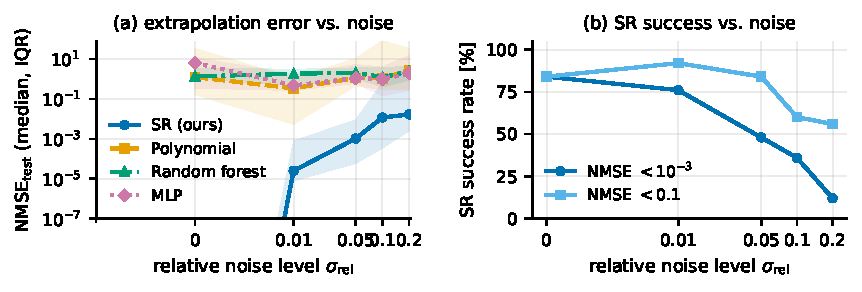
\includegraphics[width=0.94\linewidth]{../results/figs/noise.pdf}
  \caption{Noise experiment ($d{=}1$, $\mathcal{O}_{\mathrm{full}}$, $25$
  formulas per level). (a)~Median $\nmse_{\mathrm{test}}$ (values below the
  axis are exact). (b)~SR success rates at two thresholds.}
  \label{fig:noise}
\end{figure}

Figure~\ref{fig:noise} adds label noise $\sigma =
\sigma_{\mathrm{rel}}\,\mathrm{std}(f(X))$. \emph{Exact} recovery
immediately drops to zero for any $\sigma > 0$, which is unavoidable since
the fitted constants inherit an $O(\sigma)$ error, so the interesting
quantity is the test error: SR's median $\nmse$ degrades gracefully from $0$
over $10^{-3}$ ($\sigma_{\mathrm{rel}} = 0.05$) to $0.017$ at
$\sigma_{\mathrm{rel}} = 0.2$, while every baseline sits between $0.3$ and
$6.6$ across all noise levels. At $20\%$ noise our median error is still two
orders of magnitude below the best baseline. The fraction of
near-perfect extrapolations ($\nmse < 10^{-3}$) falls from $76\%$ at
$\sigma_{\mathrm{rel}} = 0.01$ to $12\%$ at $0.2$, whereas the fraction of
usable ones ($\nmse < 0.1$) only falls from $92\%$ to $56\%$: noise
therefore degrades the \emph{precision} of the recovered law much faster
than its \emph{shape}.

\subsection{Model-selection ablation}
\label{sec:ablation}

\begin{table}[t]
  \centering
  \caption{Selection ablation ($d{=}1$, $\mathcal{O}_{\mathrm{full}}$,
  $k \in \{4,6\}$ dice operators, $120$ formulas per noise level): the same
  Pareto fronts, selected by extrapolation-shaped CV (ours), standard
  interior $3$-fold CV, or raw training MSE. Differences are assessed by
  paired Wilcoxon signed-rank tests on $\log \nmse$ resp.\ $C$ over the $120$
  shared datasets.}
  \label{tab:ablation}
  \begin{tabular}{llcccc}
\toprule
$\sigma_{\mathrm{rel}}$ & Selection & med.\ NMSE & p90 NMSE & $\Pr[\nmse > 1]$ & med.\ $C$ \\
\midrule
0 & extrap-CV & $2.8\!\cdot\!10^{-30}$ & 1.14 & 0.11 & 4 \\
0 & interior-CV & $2.8\!\cdot\!10^{-30}$ & 1.21 & 0.12 & 4 \\
0 & train-MSE & $2.8\!\cdot\!10^{-30}$ & 1.76 & 0.12 & 4 \\
\midrule
0.1 & extrap-CV & 0.025 & 31.48 & 0.27 & 6 \\
0.1 & interior-CV & 0.023 & 28.86 & 0.26 & 5 \\
0.1 & train-MSE & 0.045 & 31.34 & 0.31 & 9 \\
\bottomrule
\end{tabular}
\end{table}

Table~\ref{tab:ablation} isolates the selection step: each strategy picks
from the \emph{same} Pareto front, so any difference is due to the criterion
alone. Noise-free, all three agree on almost every dataset. Under $10\%$
noise two effects separate, of very different strength.

The \emph{parsimony} effect is large and unambiguous: cross-validated
selection never returns a more complex model than training-MSE selection and
returns a strictly simpler one on $92$ of $120$ datasets (median $C = 6$
versus $9$, $p \approx 6\cdot 10^{-17}$). Its effect on accuracy is real but
far more modest: the median error roughly halves ($0.025$ versus $0.045$)
and the blow-up rate falls from $0.31$ to $0.27$, which a paired test
supports only weakly ($52$ wins, $40$ losses, $28$ ties, with $p = 0.043$).

The \emph{fold geometry}, by contrast, has no measurable effect:
extrapolation-shaped folds win on $23$ datasets and lose on $24$, with $73$
exact ties ($p = 0.63$). The tie count explains the null result: in $61\%$ of cases both
geometries select the \emph{identical} model, because the one-standard-error
rule collapses the decision onto the complexity tie-break long before fold
differences matter. We keep the extrapolation-shaped folds as the
conceptually correct validation for the target regime, at no extra cost, but
claim no empirical advantage for them. What earns its keep is parsimony.

\subsection{Analysis of learned models}
\label{sec:analysis}

\paragraph{What the search finds.}
Recovery is judged \emph{functionally}, and the search frequently returns a
different but equivalent form: the dice-rolled $\sin(2x) - \sin(2x + 2.4)$
is found as $3.73\cos(x)\sin(x - 0.37) + 0.68$ (a product-to-sum identity,
$3.73 \approx 4\sin 1.2$), and for the cubic truth $1.61 + 1.23(x - x^2)(1.08 - x)$
the core carries only $x^3$ and the background the rest. This is the division
of labour intended by~\eqref{eq:model}, visible in the learned models.

\paragraph{Failure taxonomy.}
The $30/300$ runs with $\nmse > 0.1$ concentrate on three patterns:
(i)~\emph{Poles}: truths like $1/(x - 1.32 + \cos x)$, whose test-domain
behaviour is dominated by a singularity the training data barely samples.
(ii)~\emph{Nested non-polynomial arguments}: $\log$ or $\exp$ of rational
expressions ($\log(x - \log(x^2/1.46) - 2.05)$), which the beam only reaches through
intermediate skeletons that fit poorly on their own.
(iii)~\emph{Frequency fitting}: truths like $\sin(x + 2.83x^2)$, where the
right skeleton is found but the nonconvex constant optimization
misidentifies the frequency. Usually the selection then falls back to a
simple, poorly fitting but \emph{bounded} model rather than a wildly
extrapolating one, a consequence of validating on extrapolation horizons.

\paragraph{A blind spot of in-domain validation, and its fix.}
Cross-validation has one structural blind spot. Run without the guard
described below, the worst dataset of this study selected the core
$\log(e^{-x} - e^{e^{x}})$ and reached $\nmse = 5\cdot 10^{11}$, although
that model is unremarkable on the training box ($145$ against
$\max|y_{\mathrm{train}}| = 145$). \emph{No} in-domain fold can detect this, because
extrapolation-shaped folds still only extrapolate to the edge of the data,
never past it. We therefore add a \emph{growth guard} before selection:
candidates are evaluated on the training box dilated by $1.5$, and those
that are non-finite there or exceed $10^{6}\,\max|y_{\mathrm{train}}|$ are
dropped (if all are, the front is kept). Both thresholds are deliberately
loose (a legitimate $e^{x}$ on $[-5,5]$ grows only ${\approx}12$-fold under
this dilation), and no test data is used. The guard behaves exactly
as a safety device should: comparing the $300$-dataset grid with and without
it, $299$ selections are bit-identical and only the case above changes, its
error dropping to $4\cdot 10^{-5}$, so the worst case of the whole study
falls to $153$, at no cost in recovery.

\paragraph{Selection under noise.}
For the demo function with $5\%$ noise the Pareto front collapses at $k = 2$
and then runs flat: every model above the elbow is the correct core plus a
negligible decoration such as $+\,0.0088/\sqrt{|x|}$, bought with a
training-MSE gain in the fifth decimal place. Such terms hardly affect
$\nmse_{\mathrm{test}}$ but destroy \emph{symbolic} recovery, and no
fit-based criterion rejects them. The one-standard-error rule selects the
elbow, returning $0.504\,x\sin x + 0.102x^2 + 0.0006x - 0.013$.

\section{Discussion}
\label{sec:discussion}

We built a symbolic regressor around three ideas: an unbiased
search~\citep{Kahlmeyer} made systematic by complexity-ordered enumeration
over canonical skeletons, a polynomial background whose coefficients are
projected out in closed form so that partial explanations of the data are
visible to the search early, and model selection that validates the way the
model will be used, namely on extrapolation horizons, with a
one-standard-error preference for simplicity. Its hyperparameters, including the choice between
two search configurations per dataset, are set by cross-validation. On
dice-rolled ground truths this recovers $85\%$ of formulas exactly and beats
the baselines by many orders of magnitude. Their failure is structural
(constant or linear extrapolation, degree-driven divergence) and no tuning fixes it.

Not every component earned its keep equally. The polynomial background is
decisive (recovery is non-decreasing in its degree, and cutting it back to
plain linear scaling slows the search tenfold), and so is the parsimony
rule. The extrapolation-shaped folds, however, are \emph{not} measurably
better than ordinary interior folds ($p = 0.63$): they cost nothing and are
the conceptually right validation for the target regime, but the
one-standard-error rule dominates the decision long before fold geometry
matters.

The limits of Section~\ref{sec:limits} survive: deeper enumeration with
deduplication pushed the complexity wall back but did not remove it, and even
the final configuration recovers only $41\%$ of the ground truths with
$\eff \ge 7$. More fundamentally, SR only pays off if the data-generating
process \emph{is} a formula over the chosen alphabet. Otherwise it
degrades into an expensive, poorly-behaved regressor, and a black-box model
with honestly constant extrapolation may be preferable. Natural extensions follow from these limits: the variable augmentation
of~\citet{Kahlmeyer} for divide and conquer, a core-term deletion test for
Occam behaviour under noise, and neural guidance of the
beam~\citep{ParFam}.

\clearpage
\bibliographystyle{plainnat}
\bibliography{references}
\end{document}
